

\documentclass[a4paper,12pt]{jarticle}

\newcommand{\setcounters}[1] {
  \setcounter{equation}{#1}
  \setcounter{figure}{#1}
  \setcounter{table}{#1}
}

\newcommand{\unit}[1] {
  \hspace{1mm}\mathrm{[#1]}
}

\newcommand{\degc} {
  \hspace{1mm}\mathrm{[}{}^\circ\mathrm{C]}
}

\newcommand{\refig}[1]{Fig.\ref{fig::#1}}
\newcommand{\refeq}[1]{式(\ref{eq::#1})}
\newcommand{\reftab}[1]{Tab.\ref{tab::#1}}

\newcommand{\fig}[5] {
  \begin{figure}[#1]
    \begin{center}
      \includegraphics[width=#2\hsize]{#3}
    \end{center}
    \caption{#4}
    \label{fig::#5}
  \end{figure}
}

\makeatletter
\def\eq{\@ifstar\@eq\@@eq}
\def\@eq#1{\begin{equation*}#1\end{equation*}}
\def\@@eq#1#2{\begin{equation}#2\label{eq::#1}\end{equation}}
\makeatother

\newcommand{\diff}[2] {
  \frac{\mathrm{d}#1}{\mathrm{d}#2}
}

\newcommand{\pdiff}[2] {
  \frac{\partial #1}{\partial #2}
}


\newcommand{\ddt}[2][1] {
  \ifnum #1 < 2
    \frac{\mathrm{d}#2}{\mathrm{d}t}
  \else
    \frac{\mathrm{d}^#1#2}{\mathrm{d}t^#1}
  \fi
}

\newcommand{\e}[1] {
  \mathrm{e}^{#1}
}

\newcommand{\lparen}{(}
\catcode `( = \active
\newcommand{(}{\ifmmode\left\lparen\else\lparen\fi}

\newcommand{\rparen}{)}
\catcode `) = \active
\newcommand{)}{\ifmmode\right\rparen\else\rparen\fi}

\newcommand{\bmat}[1] {
  \begin{bmatrix} #1 \end{bmatrix}
}

% -- Package ---------------------------------------------------
\usepackage{fancyhdr}
\usepackage{here}
\usepackage{listings}
\usepackage[dvipdfmx]{graphicx}
\usepackage{amsmath,amssymb,epsfig}
\usepackage{eucal}
\usepackage{bm}
\usepackage{ascmac}
\usepackage{pifont}
\usepackage{multirow}
\usepackage{enumerate}
\usepackage{cases}
\usepackage{type1cm}
\usepackage{cancel}
\usepackage{url}
\usepackage{cite}
\usepackage{color}
%\usepackage[dvipdfmx]{color}
\usepackage{caption}
\usepackage[caption=false]{subfig}
\captionsetup[figure]{labelsep=space}
\usepackage[ruled,vlined]{algorithm2e}
\usepackage{setspace}
\usepackage{comment}
\DeclareRelationFont{JY1}{mc}{it}{}{OT1}{cmr}{it}{}
\DeclareRelationFont{JT1}{mc}{it}{}{OT1}{cmr}{it}{}
\DeclareFontShape{JY1}{mc}{m}{it}{<5> <6> <7> <8> <9> <10> sgen*min
    <10.95><12><14.4><17.28><20.74><24.88> min10
    <-> min10}{}
\DeclareFontShape{JT1}{mc}{m}{it}{<5> <6> <7> <8> <9> <10> sgen*tmin
    <10.95><12><14.4><17.28><20.74><24.88> tmin10
    <-> tmin10}{}
\DeclareRelationFont{JY1}{mc}{sl}{}{OT1}{cmr}{sl}{}
\DeclareRelationFont{JT1}{mc}{sl}{}{OT1}{cmr}{sl}{}
\DeclareFontShape{JY1}{mc}{m}{sl}{<5> <6> <7> <8> <9> <10> sgen*min
    <10.95><12><14.4><17.28><20.74><24.88> min10
    <-> min10}{}
\DeclareFontShape{JT1}{mc}{m}{sl}{<5> <6> <7> <8> <9> <10> sgen*tmin
    <10.95><12><14.4><17.28><20.74><24.88> tmin10
    <-> tmin10}{}
\DeclareRelationFont{JY1}{mc}{sc}{}{OT1}{cmr}{sc}{}
\DeclareRelationFont{JT1}{mc}{sc}{}{OT1}{cmr}{sc}{}
\DeclareFontShape{JY1}{mc}{m}{sc}{<5> <6> <7> <8> <9> <10> sgen*min
    <10.95><12><14.4><17.28><20.74><24.88> min10
    <-> min10}{}
\DeclareFontShape{JT1}{mc}{m}{sc}{<5> <6> <7> <8> <9> <10> sgen*tmin
    <10.95><12><14.4><17.28><20.74><24.88> tmin10
    <-> tmin10}{}
\DeclareRelationFont{JY1}{gt}{it}{}{OT1}{cmbx}{it}{}
\DeclareRelationFont{JT1}{gt}{it}{}{OT1}{cmbx}{it}{}
\DeclareFontShape{JY1}{mc}{bx}{it}{<5> <6> <7> <8> <9> <10> sgen*goth
    <10.95><12><14.4><17.28><20.74><24.88> goth10
    <-> goth10}{}
\DeclareFontShape{JT1}{mc}{bx}{it}{<5> <6> <7> <8> <9> <10> sgen*tgoth
    <10.95><12><14.4><17.28><20.74><24.88> tgoth10
    <-> tgoth10}{}
\DeclareRelationFont{JY1}{gt}{sl}{}{OT1}{cmbx}{sl}{}
\DeclareRelationFont{JT1}{gt}{sl}{}{OT1}{cmbx}{sl}{}
\DeclareFontShape{JY1}{mc}{bx}{sl}{<5> <6> <7> <8> <9> <10> sgen*goth
    <10.95><12><14.4><17.28><20.74><24.88> goth10
    <-> goth10}{}
\DeclareFontShape{JT1}{mc}{bx}{sl}{<5> <6> <7> <8> <9> <10> sgen*tgoth
    <10.95><12><14.4><17.28><20.74><24.88> tgoth10
    <-> tgoth10}{}
\DeclareRelationFont{JY1}{gt}{sc}{}{OT1}{cmbx}{sc}{}
\DeclareRelationFont{JT1}{gt}{sc}{}{OT1}{cmbx}{sc}{}
\DeclareFontShape{JY1}{mc}{bx}{sc}{<5> <6> <7> <8> <9> <10> sgen*goth
    <10.95><12><14.4><17.28><20.74><24.88> goth10
    <-> goth10}{}
\DeclareFontShape{JT1}{mc}{bx}{sc}{<5> <6> <7> <8> <9> <10> sgen*tgoth
    <10.95><12><14.4><17.28><20.74><24.88> tgoth10
    <-> tgoth10}{}
\DeclareRelationFont{JY1}{gt}{it}{}{OT1}{cmr}{it}{}
\DeclareRelationFont{JT1}{gt}{it}{}{OT1}{cmr}{it}{}
\DeclareFontShape{JY1}{gt}{m}{it}{<5> <6> <7> <8> <9> <10> sgen*goth
    <10.95><12><14.4><17.28><20.74><24.88> goth10
    <-> goth10}{}
\DeclareFontShape{JT1}{gt}{m}{it}{<5> <6> <7> <8> <9> <10> sgen*tgoth
    <10.95><12><14.4><17.28><20.74><24.88> tgoth10
    <-> tgoth10}{}
\endinput
%%%% end of jdummy.def



% -- Margin Config ---------------------------------------------
\addtolength{\topmargin}{-\headheight}
\addtolength{\topmargin}{-\headsep}
\addtolength{\textheight}{-60truemm}

% -- Layout Config ---------------------------------------------
\setlength{\hoffset}{0cm}
\setlength{\oddsidemargin}{-3mm}
\setlength{\evensidemargin}{-3cm}
\setlength{\marginparsep}{0cm}
\setlength{\marginparwidth}{0cm}
\setlength{\textheight}{24.7cm}
\setlength{\textwidth}{17cm}
\setlength{\topmargin}{-45pt}



% -- Renewcommand ----------------------------------------------
\renewcommand{\theequation}{\arabic{section}.\arabic{equation}}
\renewcommand{\thefigure}{\arabic{figure}}
\renewcommand{\thetable}{\thesection.\arabic{table}}
\renewcommand{\lstlistingname}{ソースコード}
\renewcommand{\headrulewidth}{0mm} % fancy
\renewcommand{\labelenumi}{(\arabic{enumi})}
\renewcommand{\baselinestretch}{1.3}
\renewcommand{\floatpagefraction}{1}
\renewcommand{\topfraction}{1}
\renewcommand{\bottomfraction}{1}
\renewcommand{\textfraction}{0}
\renewcommand\thefootnote{\arabic{footnote})}
\renewcommand{\figurename}{Fig.}
\renewcommand{\tablename}{Tab.}



% -- Config for fancy package ----------------------------------
\pagestyle{fancy}
\rhead{\thepage}
\lhead{}
\cfoot{}


% -- Config for counter ----------------------------------------
\setcounter{section}{0}
\setcounter{subsection}{0}
\setcounter{subsubsection}{0}
\setcounter{equation}{0}

% 式番号を式(章番号.番号)に
\makeatletter
\renewcommand{\theequation}{\arabic{section}.\arabic{equation}}
\@addtoreset{equation}{section}
\makeatother


% -- Config for package listings -------------------------------
\lstset{
  basicstyle={\ttfamily \small},
  breaklines=true,
  frame=trBL,
  numbers=left,
  numberstyle={\ttfamily \small},
}



% 表紙
\title{卒業論文\\
早戻り機構を有するロボットハンドへの柔軟指の導入\\
% {\large No title}
}
\author{\vspace{90mm}\\
指導教員:\ 西田 \hspace{0mm} 健 准教授\\
九州工業大学\ \hspace{0mm} 工学部\\
機械知能工学科\ \hspace{0mm} 知能制御工学コース \\
\vspace{0mm}\\
学籍番号:\ 15104026\\
提出者氏名:\ 川崎 \hspace{0mm} 雄太朗\\\vspace{5mm}\\ }
\date{平成31年\ 2月\ 13日}

\begin{document}

\titlepage
\maketitle
\thispagestyle{empty}
\newpage

% 目次
\thispagestyle{empty}
\begin{abstract}

現在,産業用ロボットは多種多様な作業を遂行するためにエンドエフェクタの交換をおこなっている.
把持や運搬,組み付け作業を行うときのものをグリッパと呼ばれ,対象物の姿勢や形状に合わせて適切なグリッパへの交換が一般的に行われている.
しかし,グリッパの交換には複雑な把持計画や交換作業が伴い効率的な作業の障害となる問題が存在する.
また自動車部品の製造工場などでは上記の問題に加えて車種固有の意匠部品などは形状の多岐に及んでいるため把持の複雑さや部品自体がデリケートなものによることから従業員の手作業で組み付けが行われており,自動化できていない課題がある.\par
こうした問題を解決するために近年把持対象物の姿勢認識とグリッパの交換を省略し,作業効率を向上させるユニバーサルグリッパと呼ばれるものの開発が行われている.
ユニバーサルグリッパの中でも把持部に柔軟性のあるグリッパは,把持対象物を包み込むことで把持部を対象物に密着させて接触面積を増やし,対象物との間に生じる摩擦を増やして柔軟な把持を可能にする.
また,はや戻り機構を有するグリッパは高速で把持と開放を高速で行うことができタクトタイムの減少を期待できる.\par
本研究では,柔軟な把持を可能にする指をもちはや戻り機能を有するグリッパの提案をする.


\end{abstract}
\thispagestyle{empty}

\newpage
\tableofcontents
% 最初のやつ

\newpage
\section{序論}
\label{sec:序論}
産業用ロボットは多様な作業を遂行に対応するためにエンドエフェクタの交換がなされている.エンドエフェクタの一種にグリッパがあり対象物の把持や搬送,組み付けに利用されている.近年,グリッパの交換の省略が期待される汎用性の高いグリッパとしてユニバーサルグリッパの研究開発が行われている.\cite{end}.グリッパの交換の省略は作業環境における最適なグリッパの選定や複雑な把持計画の省略につながり作業の効率化につながる.ユニバーサルグリッパには把持面に柔軟性をもたせたグリッパの開発が進んでおり,このようなロボットに柔軟性を取り入れたソフトロボティクス\cite{soft}という学術分野が近年注目されている.\par
柔軟性のあるグリッパの例にジャミンググリッパ\cite{jam}がある.このグリッパは柔軟な半球状形袋に粒体が封入してある.このグリッパの把持方法は柔軟な状態で把持対象物に押し付け包み込んだ後エアーコンプレッサで袋内の内圧を下げることによって把持部が固化するジャミング現象を利用する.しかし,柔軟膜の耐久性や周囲の気圧などの問題があり長時間の利用が制限される.\par
半球状の柔軟膜の中にMR流体を封入したMR流体グリッパ\cite{MR}がある.
このグリッパはMR流体に磁界を印加することで粘性が変化することを応用し把持に用いる.これらのような柔軟な把持は把持対象物の形状,姿勢に左右にされない強みがある.\par
またグリッパの把持動作の高速化はタクトタイムの短縮になり,産業用ロボットの作業効率化,生産性向上につながると考えられる.指の開閉の高速化により把持動作の高速化を可能としたグリッパに早戻り機構を用いたグリッパがある\cite{sh_hand}.\par
本研究では早戻り機構を用いたグリッパに焦点を当てた.早戻り機構を有するグリッパの把持部に柔軟性をもたせることで高速な開閉が可能なグリッパに把持対象物の形状や姿勢によらない汎用性を付加可能か検証する.


\newpage
%\input{contents/structure.tex}
\newpage
\section{把持原理}
\subsection{摩擦力による把持}
本グリッパは式\ref{masatu}に示す摩擦力が把持力となり重力やその他外力とつりあうことで把持を実現する.本グリッパの指は固い円筒状の指の表面が柔軟物が取り付けてある.把持時指を対象物に接触させ力を加えていくと表面の柔軟物は対象物の形状に倣い変形する.このとき指と把持対象物の接触面積が大きくなり摩擦力が増加する.
\begin{equation}
    \label{masatu}
    F = μN
\end{equation}
\subsection{早戻り機構}
早戻り機構\cite{hayamodori}の基本的なメカニズムをレバースライダを例とし\refig{hayamodori}に示す.クランクアームA-QがQを中心に回転すると,レバーがPを中心として往復運動する.クランクアームが一定速度で回転すると点Pから離れる外側を通るときのA-B-Cの角度が240°で,内側のC-D-Aを通るときの角度が120°となりクランクアームが内側の軌道を通る時の時間は外側の軌道のものよりも短くなるので早戻り機構と呼ばれている.\par
早戻り機構を用いたグリッパは内円盤がサーボモータによって回転すると内側のボルトを軸に回転し三本の指が中央に向かって閉じる機構となっている.三本の指の動きがカメラのシャッターのように見えることからシャッターハンドと呼ばれる.指の外側の穴は小判形になっており早戻り機構の高速に動作する範囲のみを抽出できるので高速な開閉を可能にしている.シャッターハンドの開閉の様子を\refig{shutter_hand}に示す.

\begin{figure}[h]
 \begin{center}
  \includegraphics[scale=0.35]{../figure/lever.eps}
 \caption{レバースライダの例}
  \label{fig::hayamodori}
 \end{center}
\end{figure}


\begin{figure}[h]
 \begin{center}
  \includegraphics[scale=0.55]{../figure/shutterhand.eps}
 \caption{シャッターハンド}
  \label{fig::shutter_hand}
 \end{center}
\end{figure}
\newpage

	

\newpage
\section{実験}
\label{sec:実験}
\subsection{把持実験}
本グリッパの指を入れ替えて対象物の把持の可不可を検証する.指の種類はゲル,バネ,ゴムで被覆したスポンジ,柔軟物なしのものとし以下にまとめる.検証に用いる把持対象物を\refig{denso_parts}に示す.把持対象物は自動車部品工場で用いられる部品のモデルの5種類とし,それぞれA,B,C,D,Eの記号を部品ごとに割り振った.
また,把持対象物Eは\refig{E}上部の突起部と下部の外周部でそれぞれ把持実験を行った.



\subsubsection{実験手順}

\begin{enumerate}
  \item 上記の把持対象物を作業台に配置した.  
  \item グリッパの指を開き作業台の鉛直上方向から把持に適切な位置まで接近させた. 
  \item グリッパの指を閉じ把持対象物を把持した.
  \item 把持対象物を把持したまま鉛直上方向に持ち上げることができれば把持可能,持ち上げることができなければ把持不可能と判別した.
\end{enumerate}

\begin{figure}[h]
 \begin{center}
  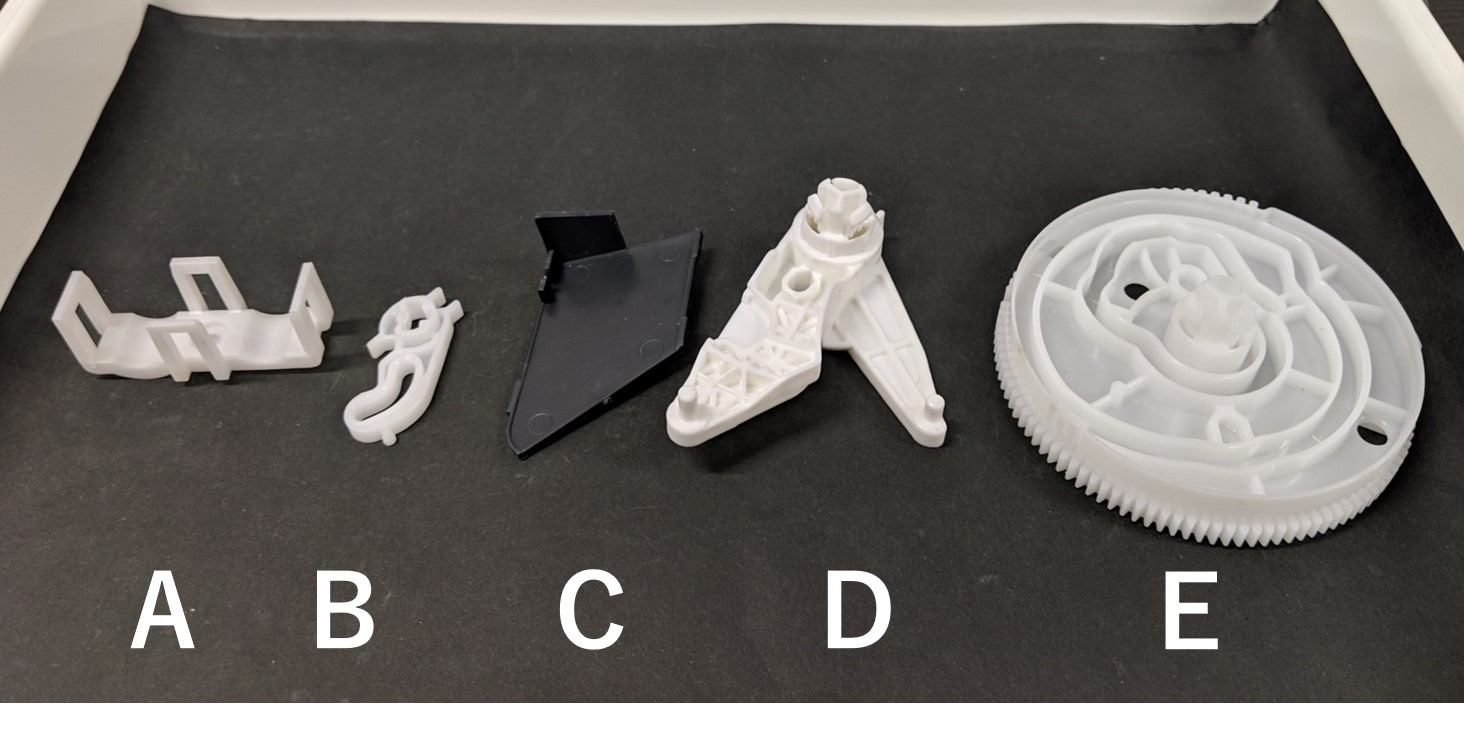
\includegraphics[scale=0.6]{../figure/denso.eps}
 \caption{自動車部品}
  \label{fig::denso_parts}
 \end{center}
\end{figure}

\begin{figure}[h]
 \begin{center}
  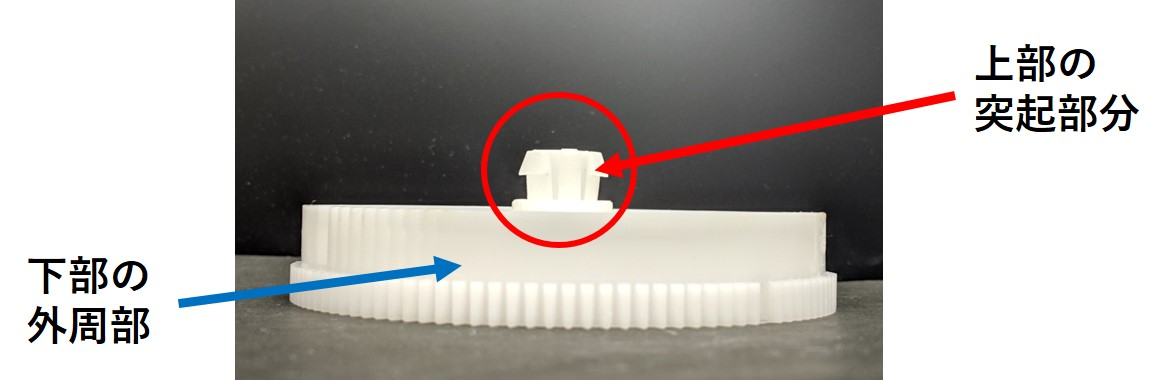
\includegraphics[scale=0.6]{../figure/E.eps}
 \caption{把持対象物E}
  \label{fig::E}
 \end{center}
\end{figure}

\newpage


\subsubsection{実験結果}
使用した指は以下の通りである.実験結果を\reftab{result}にまとめる.把持成功は◯,把持失敗は×を表している.把持対象物Eは上部の突起部と下部の外周部での把持が両方成功した時把持成功とみなした.\reftab{result}の横軸は\refig{denso_parts}の割り振った記号と対応し縦軸は以下の指の番号と対応している.

\begin{enumerate}
  \item 柔軟物のない指
  \item 厚さ3mmのゲルを取り付けた指
  \item 厚さ6mmのゲルを取り付けた指
  \item 厚さ9mmのゲルを取り付けた指
  \item 厚さ6mmのゴムで覆ったスポンジを取り付け指
  \item 厚さ8mmのゴムで覆ったスポンジを取り付け指
  \item 厚さ10mmのゴムで覆ったスポンジを取り付け指
  \item 内径6mmのばねを取り付けた指
  \item 内径7mmのばねを取り付けた指
  
\end{enumerate}

\begin{table}[htbp]
    \caption{把持実験結果}
   \label{tab::result}
   %\scalebox{3}[1.5]
   \centering
   \begin{tabular}{|c||c|c|c|c|c|} \hline
          &A    &B     &C      &D     &E        \\ \hline \hline
        (1) & ◯ & ◯  & ×  & ◯ & ×  \\ \hline
        (2) & ◯ & ◯  & ◯  & ◯ & ◯  \\ \hline
        (3) & ◯ & ◯  & ◯  & ◯ & ◯  \\ \hline
		(4) & ◯ & ◯  & ◯  & ◯ & ×  \\ \hline
		(5) & ◯ & ◯  & ◯  & ◯ & ×  \\ \hline				
		(6) & ◯ & ◯  & ◯  & ◯ & ×  \\ \hline
		(7) & ◯ & ◯  & ◯  & ◯ & ×  \\ \hline
		(8) & × & ×  & ×  & × & ×  \\ \hline		
		(9) & × & ×  & ×  & × & ×  \\ \hline		
			
		
    \end{tabular}
\end{table}

\begin{figure}[h]
\centering
\subfloat[把持対象物A]{\includegraphics[scale=0.4]{../figure/result_a.eps}}
\hspace{5mm}
\subfloat[把持対象物B]{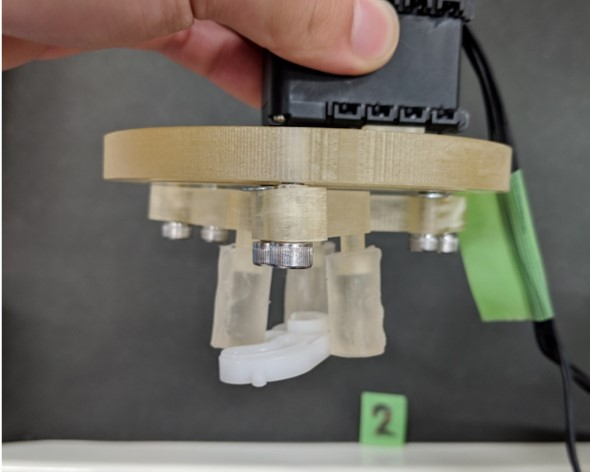
\includegraphics[scale=0.4]{../figure/result_b.eps}}
\hspace{5mm}
\subfloat[把持対象物C]{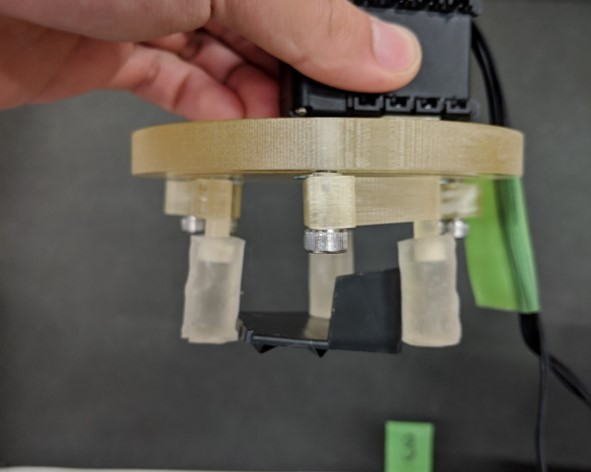
\includegraphics[scale=0.4]{../figure/result_c.eps}}
\hspace{5mm}
\subfloat[把持対象物D]{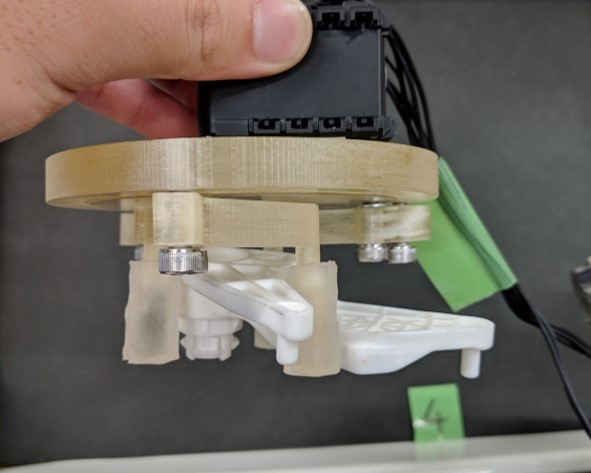
\includegraphics[scale=0.4]{../figure/result_d.eps}}
\hspace{5mm}
\subfloat[把持対象物E 上部の突起]{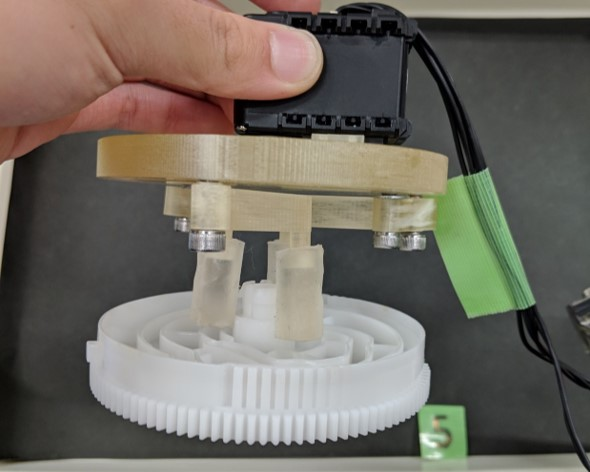
\includegraphics[scale=0.4]{../figure/result_e1.eps}}
\hspace{5mm}
\subfloat[把持対象物E 下部の外周部]{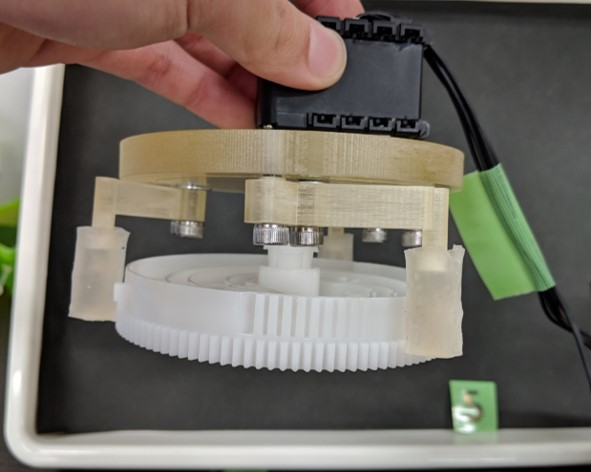
\includegraphics[scale=0.4]{../figure/result_e2.eps}}
\hspace{5mm}
\caption{厚さ3mmのゲルの指での把持の様子}
\label{fig::sisaku}
\end{figure}



\newpage
\section{考察}
柔軟物の無い指では把持対象物C,Eが把持できなかった.把持対象物の形状に倣いによって摩擦力を大きくすることの不可能な柔軟で無い指では薄い板状の把持対象物Cでは接触面積が小さすぎるため把持できなかったと考えられる.把持対象物Eに関しても同様の理由で把持できなかったと考えられる.\par
ゲルを指先に取り付けた指は厚さが3mmと6mmの場合が全ての対象物が把持出来た.厚さが9mmの指では把持対象物Eの上部の突起部分をつまむことは出来た (\refig{gel_tumami}) が外周部の把持は出来なかった.この理由はゲルの厚さが9mmと比較的指が太くなってしまい指の開きが狭くなり指を把持対象物に接触できなかったからである.ゲルの厚さを厚くすると指の開きが狭くなるのでゲルの厚さは薄くするのが望ましいと考えられる.しかし,ゲルを薄くすると把持対象物に倣う接触面積が小さくなり把持力が低下が考えられる.本実験では最もゲルの厚さが薄い3mmの指での把持は安定していた.これよりゲルの厚さ3mmの時に把持力は低下しないと考えられる.よって3mmより薄く把持が安定する厚さの検証を今後の課題とする.\par
ゴムで覆ったスポンジを取り付けた指では,全ての厚さで把持対象物A,B,C,Dは把持出来,把持対象物Eは把持できなかった.把持対象物Eの上部をつまむ把持は全ての厚さの指で出来なかった.外周部の把持は厚みが8mm,10mmのときは指が太さにより外周部に指が沿わず把持が不可能であった.厚みが6mmのときは外周部に指を沿わすことは可能だが把持は不可能であった.この理由は把持力が不足していたためであると考えられる.把持力を大きくするためにスポンジを覆うゴムをより摩擦係数の大きなゴムに変更することが有効であると考えられる.\par
ばねを取り付けた指は全ての把持対象物を把持出来なかった.ばねの指が柔軟すぎる故に外側に反り返ってしまい把持対象物に倣うことが出来ず把持力が著しく不足しているためであると考えられる.本グリッパで用いたばねよりもより固いばねを使用すれば外側への反り返りが改善され把持が可能になると考えられる.

\begin{figure}[h]
 \begin{center}
  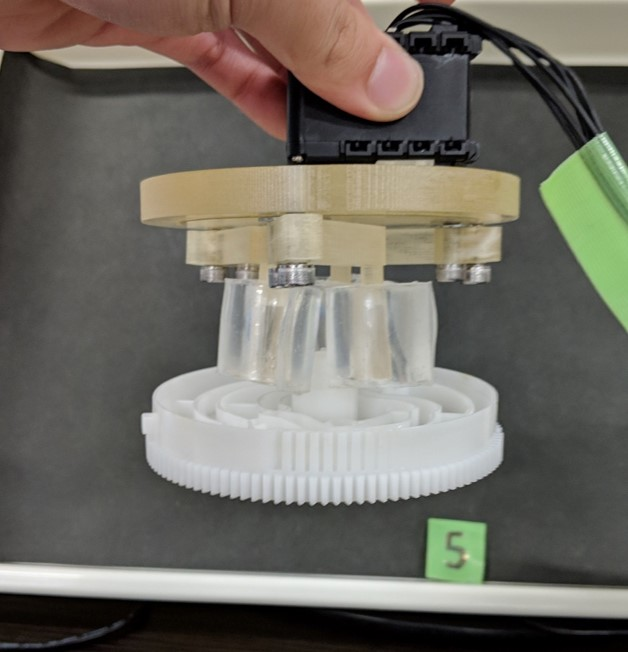
\includegraphics[scale=0.4]{../figure/gel_tumami.eps}
 \caption{厚さ9mmのゲルの指による把持対象物Eのつまみ把持}
  \label{fig::gel_tumami}
 \end{center}
\end{figure}



\newpage
\section{まとめ}
\label{sec:まとめ}
本論文では早戻り機構のグリッパの指に柔軟物を取り付け


% 謝辞
\section*{謝辞}
本論文作成にあたり御指導下さった九州工業大学大学院工学研究院機械知能工学研究系知能制御工学部門西田准教授に深く感謝致します.




\begin{thebibliography}{99}
\addcontentsline{toc}{section}{参考文献}

\bibitem{end} Tetsuyou Watanabe, Kimitoshi Yamazaki, Yasuyoshi Yokoko-hji, “Survey of robotic manipulation studies intending practi-cal applications in real environments -object recognition, softrobot hand, and challenge program and benchmarking-” , Advanced Robotics , Vol. 31, Iss. 19–20, pp. 1114-1132, 2017.
\bibitem{soft} 中村太郎,”生物・生体の機能を規範としたソフトロボティクス”,システム/制御/情報, 61巻, 7号, pp.265-270, 2017.

\bibitem{jam}J. R. Amend Jr, E. Brown, N. Rodenberg, H. M. Jaeger, H. Lipson: “A Positive Pressure
Universal Gripper Based on the Jamming of Granular Material,” IEEE trans. on Robotics,
Vol.28, pp.341–350, 2012.

\bibitem{MR}T . Nishida , Y . Okatani , K . Tadakuma ,
“ Development of universal robot gripper using
MR α fluid, ” Int . Journal of Humanoid Robotics , vol.13 ,No.4 ,p13,2016.

\bibitem{sh_hand} 天呑将成,鈴木陽介,辻徳生,渡辺哲陽,”はや戻り機構を用いた高速グリッパの開発", SICE, 2018.

\bibitem{hayamodori} 熊谷英樹,”必携「からくり設計」メカニズム定石集”,日刊工業新聞社,p140,2017.

\bibitem{gel} 柴山充弘,”ゲルの物理と化学の新展開”,日本物理学会誌 Vol 72,No.4,2017, pp.226-227, 2017.








  %\bibitem{Muhammad} Raúl Mur-Artal, J. M. M. Montiel and Juan D. Tardós. ORB-SLAM: A Versatile and Accurate Monocular SLAM System. IEEE Transactions on Robotics, vol. 31, no. 5, pp. 1147-1163, 2015.
  

%\bibitem{OSRF} ”Open Robotics", https://www.osrfoundation.org/.
%\bibitem{ROS_book}"西田健,森田賢,岡田浩之,原祥堯,山崎公俊,田向権,垣内洋平,大川一也,斎藤功,田中良道,有田裕太,石田祐太郎","実用ロボット開発のためのROSプログラミング.”,森北出版株式会社,pp.1-2, 2018.  
%\bibitem{ROS_book_PCL}"西田健,森田賢,岡田浩之,原祥堯,山崎公俊,田向権,垣内洋平,大川一也,斎藤功,田中良道,有田裕太,石田祐太郎","実用ロボット開発のためのROSプログラミング.”,森北出版株式会社,pp.5, 2018.  


\end{thebibliography}

% 付録の始まり
\appendix
%\def\thesection{付録\Alph{section}}
%\def\thesubsection{\Alph{section}\arabic{subsection}}

%\makeatletter
%\renewcommand{\theequation}{\Alph{section}.\arabic{equation}}
%\@addtoreset{equation}{section}
%\makeatother
% \setcounter{page}{1}
% ODEの説明
%\section{ }
%\label{sec:}


% % 図の挿入

% \begin{figure}[b]
%  \begin{center}
%   \includegraphics[scale=0.9]{../figure/circuit.eps}
%   \caption{Uncontrolled converter}
%   \label{circuit}
%  \end{center}
% \end{figure}


% % 表の挿入

% \begin{table}[htb]
%   \begin{center}
%     \caption{各素子のパラメータ}
%     \begin{tabular}{c|c|c} \hline
%       定数名[単位] & 記号 & 値 \\ \hline \hline
%       周波数[Hz] & $f_U,f_V,f_W$ & 120 \\ \hline
%                      & $\phi_U$ & $\frac{2\pi}{3}$ \\
%       初期位相角[rad] & $\phi_V$ & $\frac{4\pi}{3}$ \\
%                      & $\phi_W$ & $2\pi$ \\ \hline
%       抵抗[$\Omega$] & $R$ & 10 \\ \hline
%     \end{tabular}
%     \label{param}
%   \end{center}
% \end{table}


% % 図の挿入

% \begin{figure}[tb]
%  \centering
%  \vspace{0.5cm}
%  \includegraphics[scale=0.85]{../figure/waves.eps}\\
%  \hspace{0.0cm}
%  % 入力と出力\\
%  % \\
%  % \vspace{1.2cm}
%  % \includegraphics[scale=0.825]{../figure/output.eps}\\
%  % (b) 出力の電位\\
%  % \\
%  \caption{シミュレーションにより得られた各電源電圧(上)と出力電位(下)の波形}
%  \label{wave}
% \end{figure}

% \newpage

% % 図を並べて挿入

% \begin{figure}[tb]
%  \centering
%  \subfloat[区間1における回路動作]{\includegraphics[scale=0.5]{../figure/kukan_1.eps}}
%  \hspace{1.5cm}
%  \subfloat[区間2における回路動作]{\includegraphics[scale=0.5]{../figure/kukan_2.eps}}
% \\
%  \vspace{0.5cm}
%  \subfloat[区間3における回路動作]{\includegraphics[scale=0.5]{../figure/kukan_3.eps}}
%  \hspace{1.5cm}
%  \subfloat[区間4における回路動作]{\includegraphics[scale=0.5]{../figure/kukan_4.eps}}
% \\
%  \vspace{0.5cm}
%  \subfloat[区間5における回路動作]{\includegraphics[scale=0.5]{../figure/kukan_5.eps}}
%  \hspace{1.5cm}
%  \subfloat[区間6における回路動作]{\includegraphics[scale=0.5]{../figure/kukan_6.eps}}
% \\
%  \caption{各区間での回路動作の様子}
%  \label{circuit_kaku}
% \end{figure}

% % 文中へのラベリング
% {\bf Fig. }\ref{circuit_kaku}に示す〜



\end{document}
